\chapter{Creating the CFS model}\label{sec:cfs}
The BSDF data can be generate through several methods: window modelling software (e.g. WINDOW 7.3), simulation programs (e.g. TrancePro or Radiance's "genBSDF") or measurements with a goniophotometer. In this section will be give an overview of the BSDF file creation with the software WINDOW 7.3.\\

We will use the software WINDOW 7.3 by LBNL for the BSDF generation. The tool can be downloaded from \url{http://windows.lbl.gov/software/window/window.html}.
Firstly, adjust the optical calculation options in the software preferences, \textit{File -> Preferences}. Checking the relative boxes as shown in figure \ref{img2:preference}, WINDOW gives in output the BSDF matrices of the complete fenestration system in an xml extension. In particular, it is also possible to have in output the BSDF data for both solar and visible band, remembering that Radiance only uses the front transmission data in the visible range. 
%On the other side, for the thermal simulation it is required also the solar band. 

\begin{figure}[h]
\centering
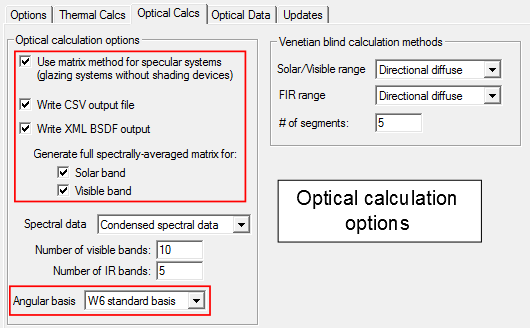
\includegraphics[width=0.7\textwidth]{preference}
\caption{\label{img2:preference} Preference setting in WINDOW 7.3}
\end{figure}

Particular attention should be paid to the angular basis option; this option defines the sky division in order to have a BSDF matrix 145x145 size, and to avoid error in the simulation. It is required to set the "W6 standard basis" (Figure \ref{img2:preference}) that correspond to the Klems division.

Once adjusted the preferences, move to the \textit{Glazing System Library} (figure \ref{img2:windowglass}) where it is possible to create the fenestration system choosing the glass and the shade typology from the respective database (IGDB and CGDB). First, create a double pan-glass low-e as in Figure \ref{img2:windowglass}, name it "2pan\_lowe" and export it following the tutorial \url{http://sel.me.wisc.edu/trnsys/downloads/tutorials_and_examples/window5/windowtutorial.pdf} in order to make available this new system in TRNSYS. Then click the Calc [F9] button in order to create the BSDF file of this system in xml extension.\\


\begin{figure}[h]
\centering
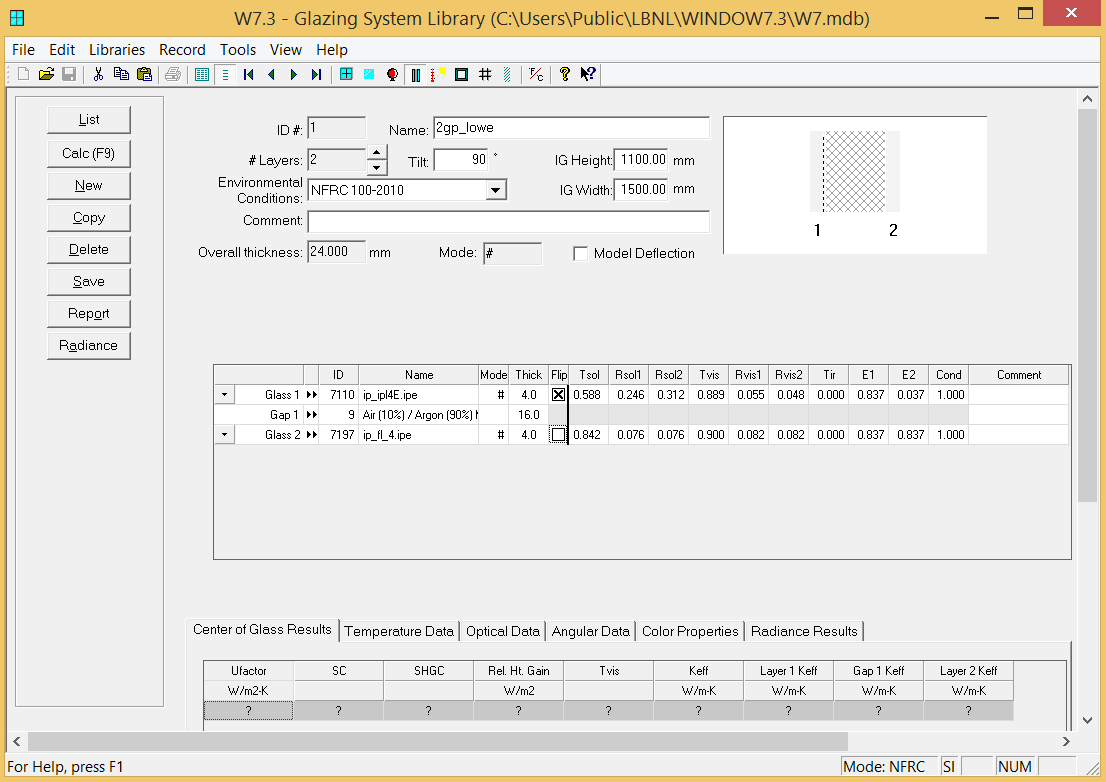
\includegraphics[width=0.9\textwidth]{windowglass}
\caption{\label{img2:windowglass} Base configuration system in Glazing System Library}
\end{figure}

In order to add the shading increase the number of layer to 3 and select "shade or frit" from the drop down list for the first (Figure \ref{img2:window73_2}).
\begin{figure}[h]
\centering
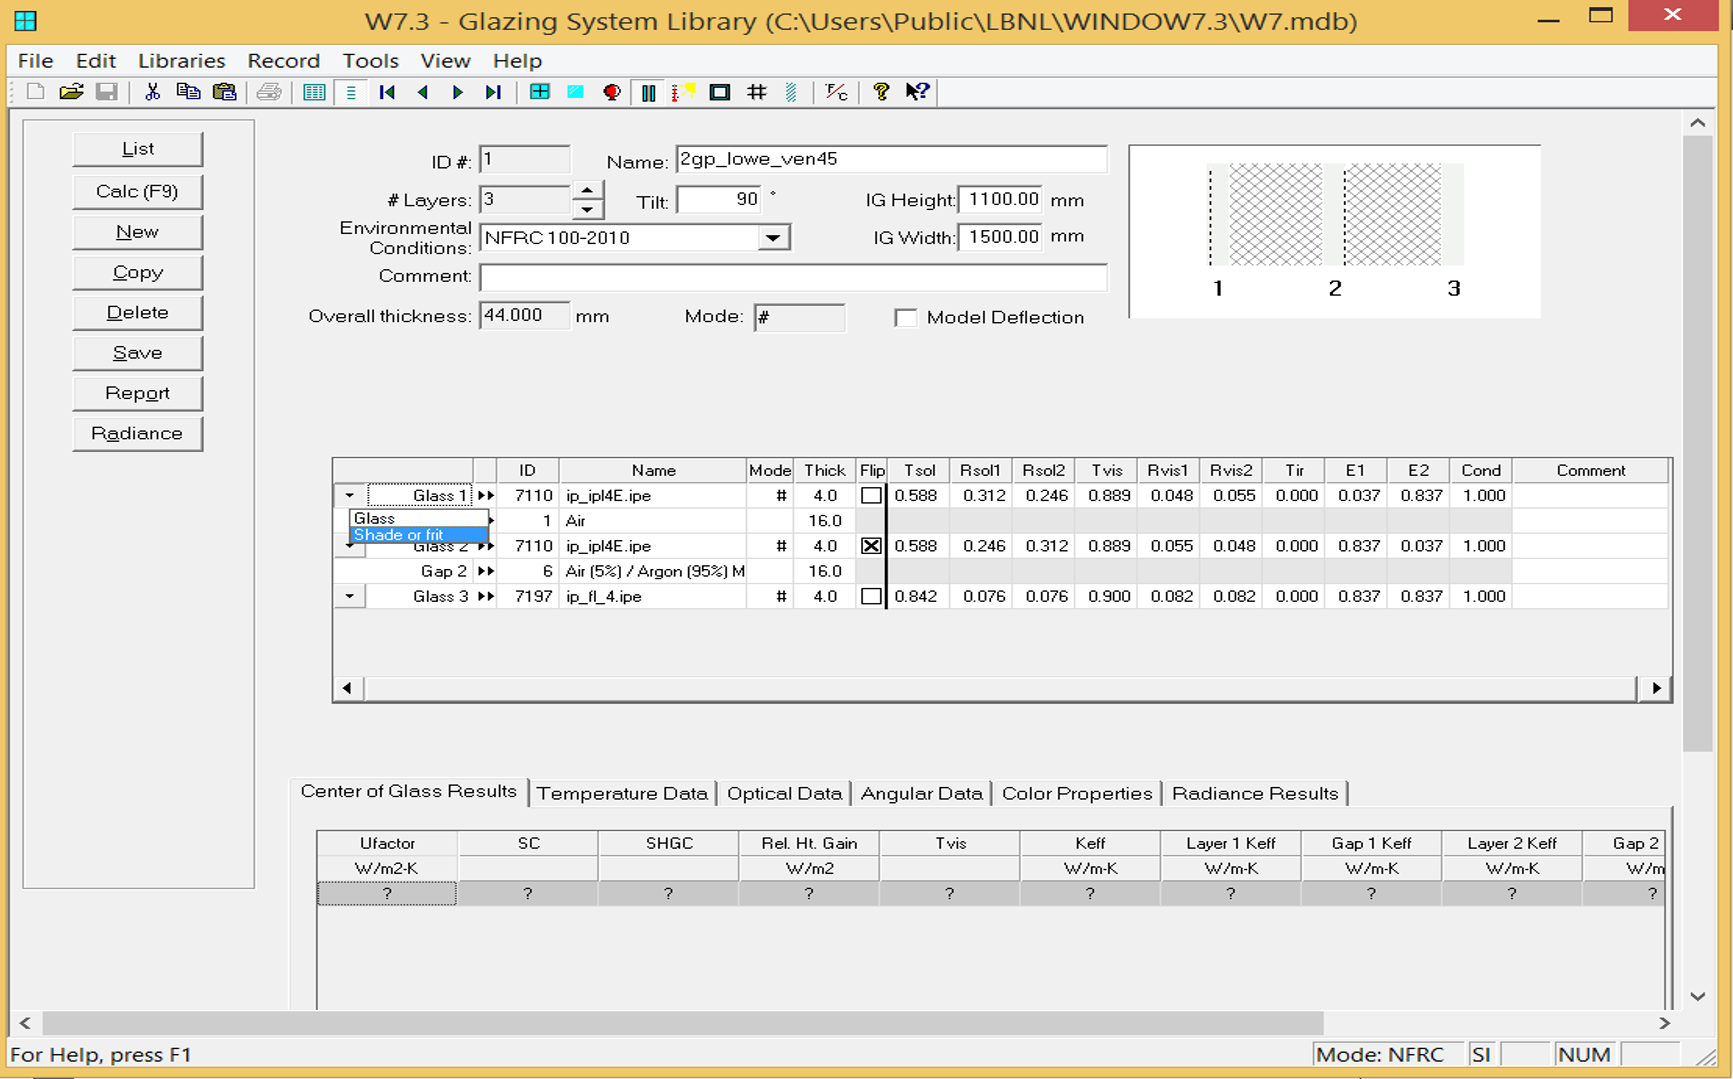
\includegraphics[width=0.9\textwidth]{window73_2}
\caption{\label{img2:window73_2} Adding the shading layer in Glazing System Library}
\end{figure}

In \textit{Shading Layer Library} (Figure \ref{img2:shading}) the shade properties can be adjusted or a new shade can be create, choosing between: venetian blinds, homogeneous diffusing shade, woven shade, fritted shade. Then, for each typology, it is possible to choose geometric and optical parameters. WINDOW allows also to use BSDF data pre-calculated in the shading type by selecting "shade with XML data". 

\begin{figure}[h]
\centering
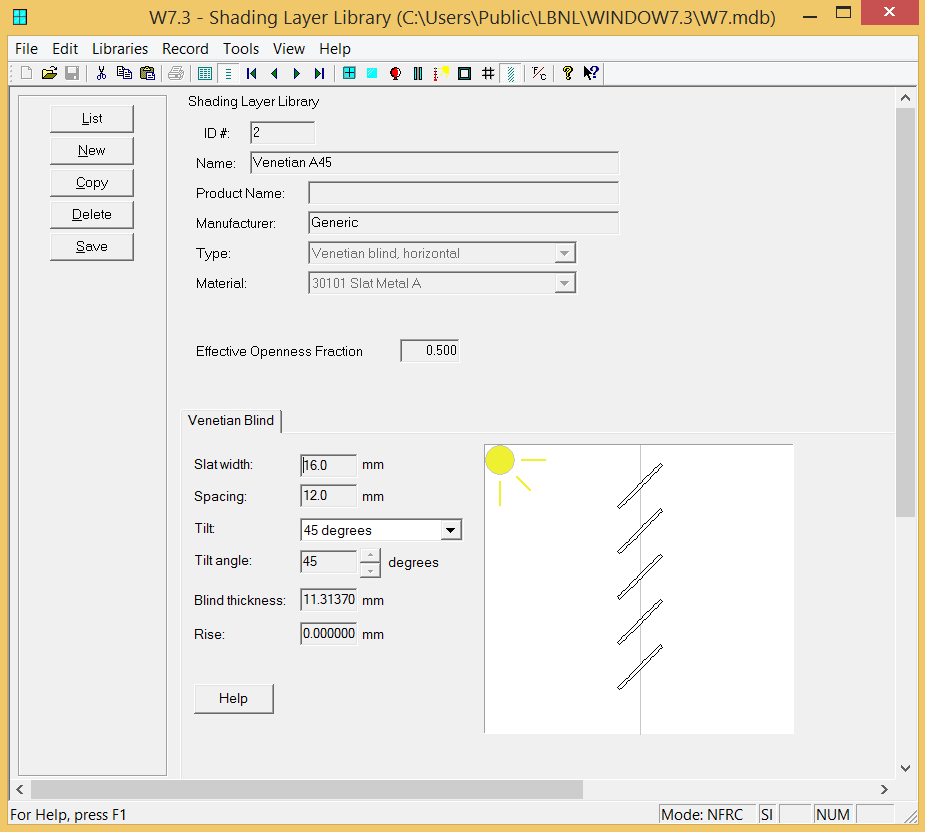
\includegraphics[width=0.9\textwidth]{shading}
\caption{\label{img2:shading} Venetian blinds configuration in Shading Layer Library}
\end{figure}

Select the shading in Figure \ref{img2:shading} for the shading layer and you will obtain a complete system as in Figure \ref{img2:window73} and name it with a name easy to recognize (e.g. 2pan\_lowe\_venetian45).

\begin{figure}[h]
\centering
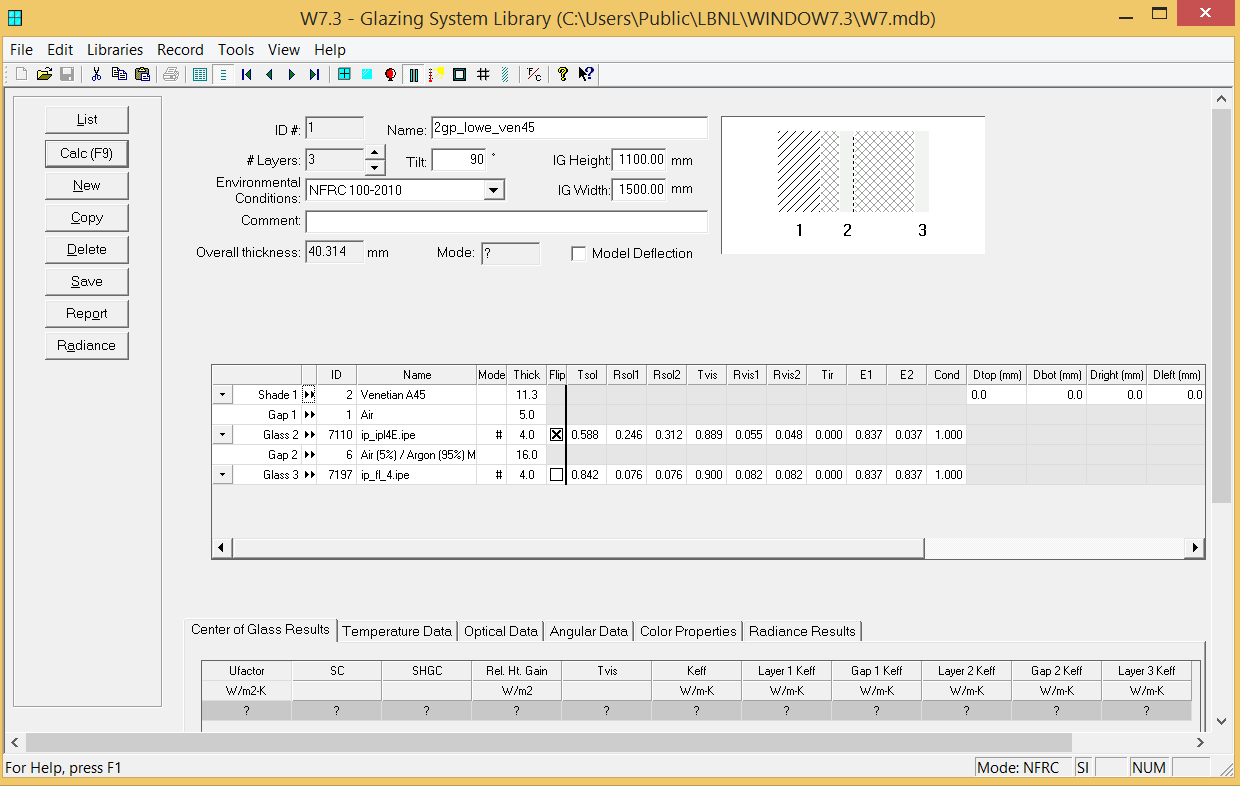
\includegraphics[width=0.9\textwidth]{window73}
\caption{\label{img2:window73} Complete glazing system in Glazing System Library}
\end{figure}

Click again the \textit{Calc} [F9] button. An xml file with the name of the system will be created in the directory
\begin{center}
\textit{C:\textbackslash Users\textbackslash Public\textbackslash LBNL\textbackslash WINDOW7.3\textbackslash BSDFs}
\end{center}

Create, with the same steps above, the BSDFs file for the configuration with blinds at 0 and 90-degree tilt angle in order to define a dynamic shading system.\\
Rename the BSDF file with a integer number starting with the number 0 that correspond to the base configuration (e.g. glass without shading) and increase the numeration starting from the more open configuration (0-degree tilt angle) to the more closer (90-degree tilt angle). \\
The BSDF file created has to be locate it in a specific folder where the TypeDLT can find it (see Chapter \ref{sec:manualtweaks}).\\